% !TEX root = ../ac_paper.tex

\section{Embeddings}

\subsection{Transformers: a review}

Previously an encoder-only transformer was used in

\subsection{BFS-easy and BFS-hard examples of Miller-Schupp series}

We consider all examples of the Miller-Schupp series for $n \leq 7$ and $\text{len}(w) \leq 7$.
We freely and cyclically reduce $x^{-1}w$ and, keep only one element of each orbit under the action of cyclic permutations.
\footnote{Here, the restriction len$(w) \leq 7$ was imposed \textit{before} freely and cyclically reducing $x^{-1}w$.
The total length of a presentation in the Miller-Schupp series before this reduction is $2n+4+\text{len}(w)$, however, after these reductions, the total length decreases to $2n+4+\text{len}(w')$ where $x^{-1}w'$ is the reduced word.
This can be a source of confusion.
Maybe I should consider all examples that satisfy $\text{len}(w') \leq 7$.}
There are 170 relators of the form $x^{-1}w$ with these restrictions, and hence 1190 presentations in total.
We use the algorithm presented in Algorithm \autoref{alg:bfs} to classify these examples as solved or unsolved.
For each presentation $R_0$, we start with a heap $H$ and a set $S$; each of them containing only $R_0$.
The heap $H$ is ordered by a tuple $(n, m)$ where $n$ is the total length of a presentation and $m$ is the length of the sequence of AC moves connecting a presentation and $R_0$.
The size of the tree grows extremely fast\footnote{Something like $n^k$?}, hence we put a hard cutoff on the number of nodes of the tree.
If the algorithm finds the trivial presentation, we consider the starting presentation $R_0$ 'BFS-easy'; else, we consider it a 'BFS-hard' example.
\footnote{Justify the BFS name.}
\footnote{Note that the choice of $10^6$ nodes is based entirely on computational convenience.
With this choice, we found that each example took 1-2 minutes to process.
For 1190 presentations, this amounted to approximately 20 hours.
Can this be made more precise maybe in terms of CPU time?}
\footnote{The sequence we first encounter depends on the choice of sequence of AC moves in the for loop.
What is that sequence in our case?}
\footnote{Isn't S a set instead of a list? Specify what Actions, H, $N_f$ mean in our case.
Why should this algorithm be called BFS?}

\begin{algorithm}
	\caption{Search algorithm}\label{alg:bfs}
	\begin{algorithmic}
		\State $H \gets R_0$ \Comment{Initialize the heap of presentations with $R_0$.}
		\State $S \gets R_0$ \Comment{Initialize the set of seen presentations with $R_0$.}

		\While{$\text{len}(S) < 10^6$} \Comment{While number of nodes in $S$ is less than $N$.}
		\State $R \gets H[0]$ \Comment{Pop the top element of the heap.}
		\For{$A \in \text{AC Moves}$}
		\State $RA \gets A \cdot R$ \Comment{Act on $R$ by $A$.}
		\If{RA is trivial}
		\Return{True}
		\Else{ $RA \notin S$}
		\State $S \gets RA$
		\State $H \gets RA$ \Comment{Add $RA$ to $H$ keeping the heap invariant.}

		\EndIf
		\EndFor
		\EndWhile
	\end{algorithmic}
\end{algorithm}

The number of BFS-hard examples increases as a function of $n$.
(See \autoref{fig:hist_vs_n}.)
The distributions of BFS-easy and BFS-hard as a function of the total length of a presentation are also given in \autoref{fig:hist_vs_length}.

\begin{figure}
	\centering
	\begin{subfigure}[b]{0.5\textwidth}
		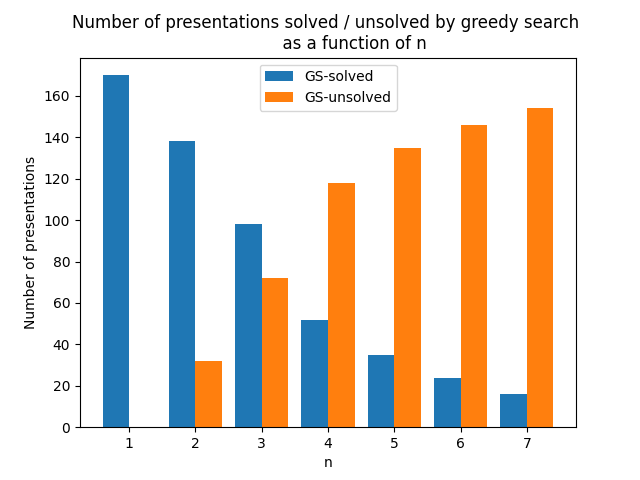
\includegraphics[width=\textwidth]{fig/hist_vs_n.png}
		\caption{Distribution versus $n$}
		\label{fig:hist_vs_n}
	\end{subfigure}%
	%add desired spacing between images, e. g. ~, \quad, \qquad etc.
	%(or a blank line to force the subfigure onto a new line)
	\begin{subfigure}[b]{0.5\textwidth}
		\centering
		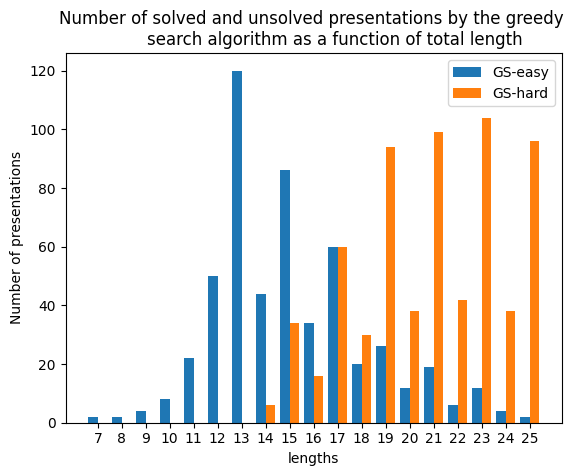
\includegraphics[width=\textwidth]{fig/hist_vs_lengths.png}
		\caption{Distribution versus total length}
		\label{fig:hist_vs_length}
	\end{subfigure}
	\caption{Number of presentations}\label{fig:miller_schupp_statistics}
\end{figure}

\subsection{Dataset for the GPT model}

We apply sequences of AC moves to the Miller-Schupp series presentations studied in the previous subsection to generate a dataset.
We use Algorithm \autoref{alg:apply_ac_moves} to ensure that the total length of the generated presentations follows roughly a uniform distribution.
(See \autoref{fig:gpt_data}; there, the distribution is roughly uniform with short tails on either side.)
\footnote{Maybe there should be only one histogram in the figure showing combined solved+unsolved statistics.
As it is, I computed separate percentages for each solved/unsolved case.
I should clarify that if I leave the figure as it is.
It is also good to change the total length.
Also change the label of x-axis to something better.}

Algorithm \autoref{alg:apply_ac_moves} generates presentations of increasing lengths in $n$ phases.
In the $i$-th phase, presentations with maximum relator length $l_i$ are generated, where $l_i$ is sampled from a discrete uniform distribution with bounds $l + i l_{\text{inc}} $ and $l + (i+1) l_{\text{inc}}$.
Here, $l$ is the maximum of the lengths of the two relators in the initial Miller-Schupp presentation $R_0$ (and thus the minimum value of maximum relator length in the algorithm), and $l_{\text{inc}}$ is defined in terms of the maximum possible relator length $l_{\text{max}}$ we wish to obtain in the last phase as $l_{\text{inc}} = (l_{\text{max}}-l)/n$.
In the $i$-the phase, $T$ AC moves are applied to a presentation generated in the $(i-1)$-th phase.
In our work, we chose $l_{\text{max}}=128$, $n=128$, $m=12$, and $T=1000$.
\footnote{Specify much earlier in the paper, and here as well, that whenever we apply AC moves, we set a maximum length up to which each relator is allowed to grow.
Any AC move that would result in a presentation of longer relator length acts trivially.
Maybe instead of writing $A \sim \text{AC Moves}$, there should be a notation like $(AC)_l$ when $l$ is specified to be the maximum relator length.}

\begin{algorithm}
	\caption{Generate AC Cousins}\label{alg:apply_ac_moves}
	\begin{algorithmic}
		\Require $R_0$, $l_{\text{max}}$, $n$, $m$, $T$
		\State $L \gets \{ \}$ \Comment{Initiate the list $L$ of all presentations}

		\State $l \gets \max(l_1, l_2)$

		\Comment{Set $l_1$, $l_2$ are the lengths of relators of $R_0$}

		\State $l_{\text{inc}} \gets (l_{\text{max}}-l)/n$

		\Comment{The increment by which the maximum relator length increases in each phase}

		\For {$i = 1, 2, \cdots, n$}

		\Comment{Loop over $n$ phases}
		\For {$j = 1, 2, \cdots, m$}

		\Comment{Generate $m$ presentations in each phase}
		\State $l_i \sim \mathcal{U}(l + i l_{\text{inc}} , l + (i+1) l_{\text{inc}})$

		\Comment{Set the maximum relator length for $i$-th phase}
		\If{i is 0}
		\State $R \gets R_0$
		\Else
		\State $R \gets L[(i-1) \times m+j]$
		\EndIf

		\Comment{Set $R$ to a presentation of the previous phase if $i > 0$, else set it to the initial presentation $R_0$}


		\For{$k = 1, 2, \cdots, T$}

		\Comment{Apply $T$ randomly selected AC-moves}
		\State A $\sim$ AC Moves
		\State $R \gets A \cdot R$

		\EndFor

		\State $L \gets R$

		\Comment{Add the resultant presentation $R$ to $L$}

		\EndFor
		\EndFor
	\end{algorithmic}
\end{algorithm}

The main reason for choosing this algorithm is so that our GPT model sees roughly the same amount of presentations of each length and is, hence, not biased towards shorter or longer presentations.
The final dataset contained 0.8 million (1 million) presentations generated from applying Algorithm \autoref{alg:apply_ac_moves} to BFS-easy (BFS-hard) examples.
Only a small amount (roughly 15 percent) of the original Miller-Schupp presentations remained to be part of this dataset.

\begin{figure}
	\centering
	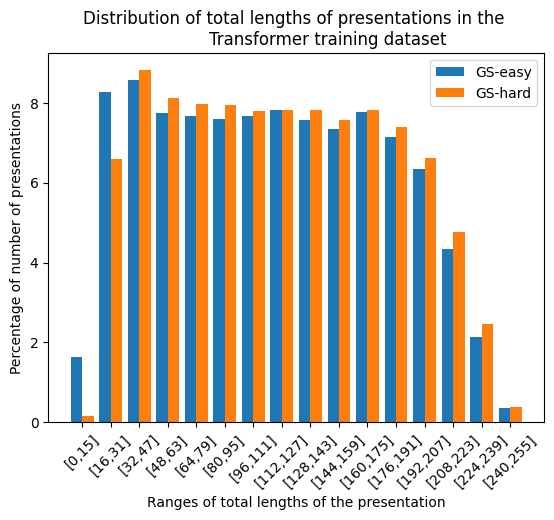
\includegraphics[scale=0.6]{fig/gpt_data_length_distribution.png}
	\caption{Percentage of presentations in various ranges of total lengths.}
	\label{fig:gpt_data}
\end{figure}

The dataset is tokenized by adding two stop tokens that represent the end of two relators of a presentation.
Thus there are six tokens in total: one each for $x$, $y$, $x^{-1}$, and $y^{-1}$ and the two stop tokens.
The tokenized dataset has about 217M tokens, and the distribution of tokens is shown in \autoref{fig:tokens_hist}.
We note that $y$ and $y^{-1}$ appear significantly more often than $x$ and $x^{-1}$ in the unsolved dataset.
This is likely because the BFS-hard examples have higher $n$, and higher $n$ corresponds to more of a presence of $y$ and $y^{-1}$.
Interestingly, this effect remains in the dataset even when we apply thousands of AC moves.
I should investigate this further.

We set aside 10 percent of the data as a validation dataset.

\begin{figure}
	\centering
	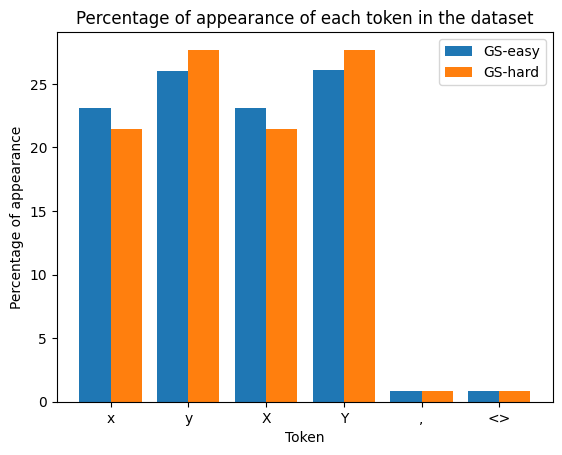
\includegraphics[scale=0.6]{fig/tokens_hist.png}
	\caption{Percentage of appearance of each token in the solved/unsolved datasets.}
	\label{fig:tokens_hist}
\end{figure}

\subsection{Results}
We train a GPT model on the dataset described in the previous subsection.
Given a context of $n$ tokens, a GPT model learns the probability distribution for $(n+1)$-st token.
The extent to which it can make good predictions is measured by a cross-entropy loss defined above.
We trained a model with embedding dimension 512 and 8 layers.
The model is initialized with random weights that assigns an equal probability to each token, thus the initial value of the cross-entropy loss is $-\ln(1/6) \sim 1.7917$.
As the model was trained, we were able to achieve the minimum validation loss of 0.5685.
\footnote{insert a validation loss curve.}

We use the trained model to obtain embeddings of the 1190 Miller Schupp presentations studied above.
To visualize these embeddings, we use t-SNE with distance measured by the cosine of the angle between two embedding vectors and project the embedding space down to two dimensions.
The final result is shown in \autoref{fig:embeddings_tsne}.
We see that the model has clustered together examples with the same $n$.

\footnote{Maybe I should replace 'Solved' and 'Unsolved' with 'BFS-easy' and 'BFS-hard' in all the images.}

\begin{figure}
	\centering
	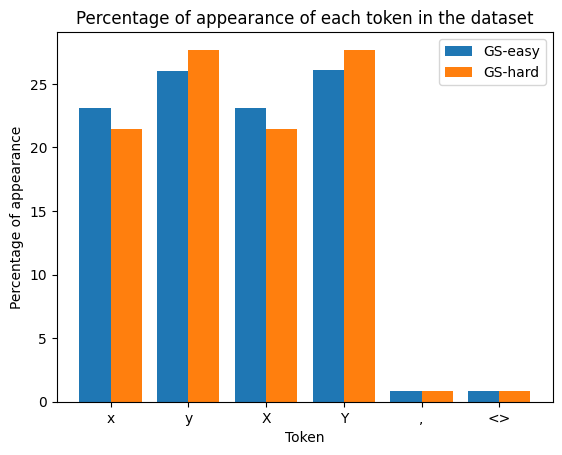
\includegraphics[scale=0.6]{fig/tokens_hist.png}
	\caption{Percentage of appearance of each token in the solved/unsolved datasets.}
	\label{fig:tokens_hist}
\end{figure}

\begin{figure}
	\centering
	\begin{subfigure}[b]{\textwidth}
		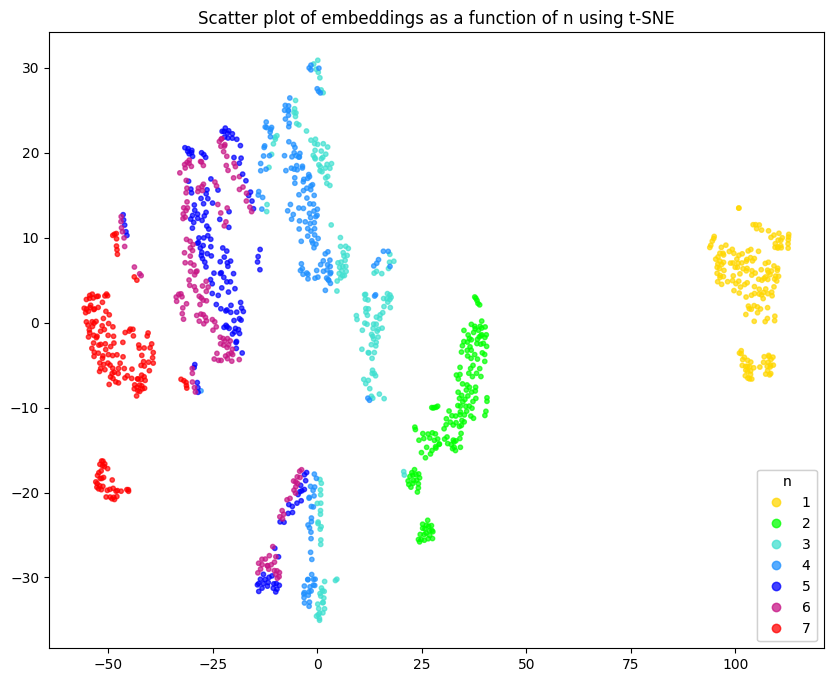
\includegraphics[width=1\linewidth]{fig/embeddings_n.png}
		\caption{Scatter plot of embeddings as a function of $n$ using t-SNE}
		\label{fig:hist_vs_n}
	\end{subfigure}%
	%add desired spacing between images, e. g. ~, \quad, \qquad etc.
	%(or a blank line to force the subfigure onto a new line)

	\begin{subfigure}[b]{\textwidth}
		\centering
		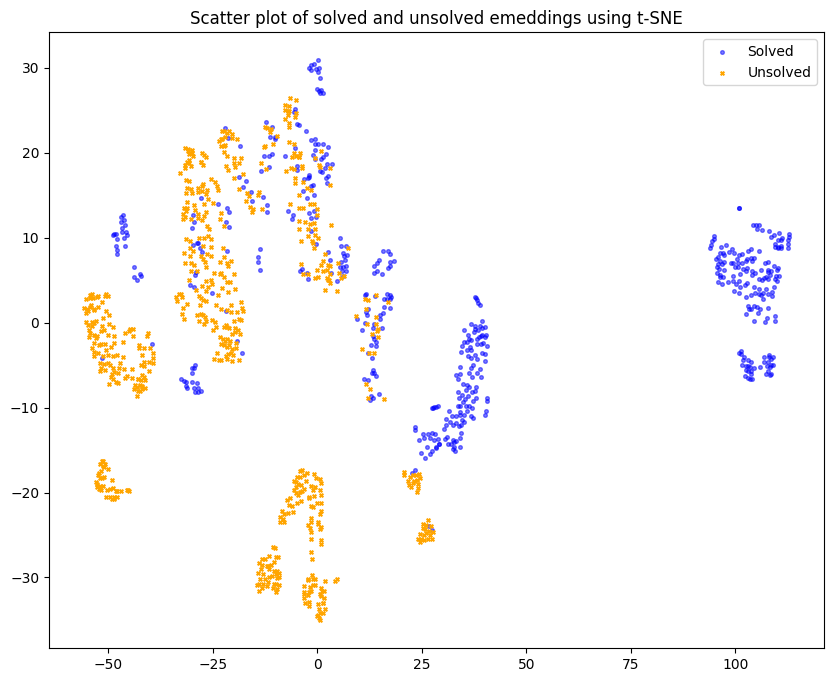
\includegraphics[width=1\linewidth]{fig/embeddings_easy_vs_hard.png}
		\caption{Scatter plot of BFS-easy and BFS-hard examples using t-SNE}
		\label{fig:hist_vs_length}
	\end{subfigure}
	\caption{Projection of embeddings to a plane using t-SNE with cosine similarities}\label{fig:embeddings_tsne}
\end{figure}